\documentclass[12pt,a4paper,openright,titlepage,twoside]{book}
\usepackage[T1]{fontenc} % codifica dei font
\usepackage[utf8]{inputenc} % lettere accentate da tastiera
% Includere pagine pdf (frontespizio)
\usepackage{pdfpages}
% tesi in italiano
\usepackage[italian]{babel}
% Margini: 3 cm sopra, sotto e sui lati 
\usepackage{geometry}
\geometry{a4paper,top=3cm,bottom=3cm,left=3cm,right=3cm,heightrounded}
% Interlinea 1.5
\usepackage{setspace}
\onehalfspacing
\raggedbottom
\usepackage{newtxtext,newtxmath}
% Numerazione pagine in basso a dx e sx e intestazione in alto
\usepackage{fancyhdr}
\pagestyle{fancy}
\renewcommand{\chaptermark}[1]{\markboth{\MakeUppercase{#1}}{}} %rimuovi l'enumerazione dei capitoli dall'intestazione
\renewcommand{\headrulewidth}{0.5pt}
\renewcommand{\footrulewidth}{0pt}
\fancyhf{}
\fancyfoot[LE,RO]{\thepage}
\fancyhead[LE,RO]{\slshape \rightmark}
\fancyhead[LO,RE]{\slshape \leftmark}
%headheight
\setlength{\headheight}{14.49998pt}
% Pagine bianche senza intestazione
\makeatletter
\def\cleardoublepage{\clearpage\if@twoside \ifodd\c@page\else
	\hbox{}
	\vspace*{\fill}
	\vspace{\fill}
	\thispagestyle{empty}
	\newpage
	\if@twocolumn\hbox{}\newpage\fi\fi\fi}
\makeatother
% sommario
\newenvironment{abstract}%
{\cleardoublepage%
	\thispagestyle{empty}% non rendo visibile la numerazione
	\null \vfill\begin{center}%
		\bfseries \abstractname \end{center}}%
{\vfill\null}
\providecommand{\abstract}{}
% Titoli
\usepackage{titlesec}
\titleformat{\chapter}[display]
{\normalfont\bfseries}{}{0pt}{\Huge}
\titlespacing*{\chapter}{0pt}{-50pt}{40pt}
% Bibliografia
\usepackage[autostyle, italian=guillemets]{csquotes}
\usepackage[backend=biber, style=numeric]{biblatex}
\usepackage{guit} 
\addbibresource{bibliografia.bib}
% Riferimenti incrociati
\usepackage[italian]{varioref}
% citazioni
\usepackage{quoting}
\quotingsetup{font=small}
%commenti
\usepackage{comment}
% Acronimi
\usepackage[printonlyused,withpage]{acronym}
% Figure
\usepackage{graphicx}
\usepackage[nottoc]{tocbibind}
\usepackage{wrapfig}
\usepackage{float}
% math
\usepackage{amsmath}
% Didascalie
\usepackage[font=small,format=hang,labelfont={sf,bf}]{caption}
\usepackage{subcaption}
% tabelle
\usepackage{tabularx}
% Codice
%\usepackage{listings}
\usepackage{listings,xcolor}
\addto\captionsitalian{%
	\renewcommand{\lstlistingname}{Codice}
	\renewcommand{\lstlistlistingname}{Elenco dei codici}}
\definecolor{codeCommentGray}{rgb}{0.55,0.55,0.55}
\definecolor{codeNaturalColorSystem}{rgb}{0,0.48,0.65}
\definecolor{codeDarkMagenta}{rgb}{0.53,0.06,0.58}
\definecolor{codeMediumDarkblue}{rgb}{0,0.20,0.70}
\definecolor{codeOliveGreen}{rgb}{0.50,0.50,0}
\definecolor{codeNumberColor}{rgb}{0.09,0.31,0.92}
\definecolor{codeDarkGreen}{rgb}{0.02,0.49,0.09}
%\definecolor{backcolour}{rgb}{0.95,0.95,0.92}
\lstdefinestyle{mystyle}{
	%	backgroundcolor=\color{backcolour},   
	commentstyle=\color{codeCommentGray},
	keywordstyle=\color{codeMediumDarkblue},
	numberstyle=\tiny, %\color{codegray},
	stringstyle=\color{codeDarkGreen},
	basicstyle=\ttfamily\footnotesize,
	breakatwhitespace=false,         
	breaklines=true,                 
	captionpos=b,                    
	keepspaces=true,                 
	numbers=left,                    
	numbersep=5pt,                  
	showspaces=false,                
	showstringspaces=false,
	showtabs=false,                  
	tabsize=2,
	frame=lines
}
%\lstset{emph={acronym,shortName,extendedName,code,correction},
	%	emphstyle=\color{codeDarkMagenta},
	%	emph={[2]Acronimo},
	%	emphstyle={[2]\color{codeNaturalColorSystem}}}
\lstset{style=mystyle}
\lstset{language=[AspectJ]Java}
\lstset{moredelim=[is][\color{codeNaturalColorSystem}]{|*}{*|}}
\lstset{moredelim=[is][\color{codeNumberColor}]{?*}{*?}}
\lstset{moredelim=[is][\color{black}]{!*}{*!}}
% Collegamenti ipertestuali e al Web
\usepackage[colorlinks]{hyperref} % sempre per ultimo
\hypersetup{
	colorlinks=true,
	linkcolor=black,
	filecolor=magenta,      
	urlcolor=cyan,
}
%\hypersetup{hidelinks}


\begin{document}
	
	\frontmatter	
	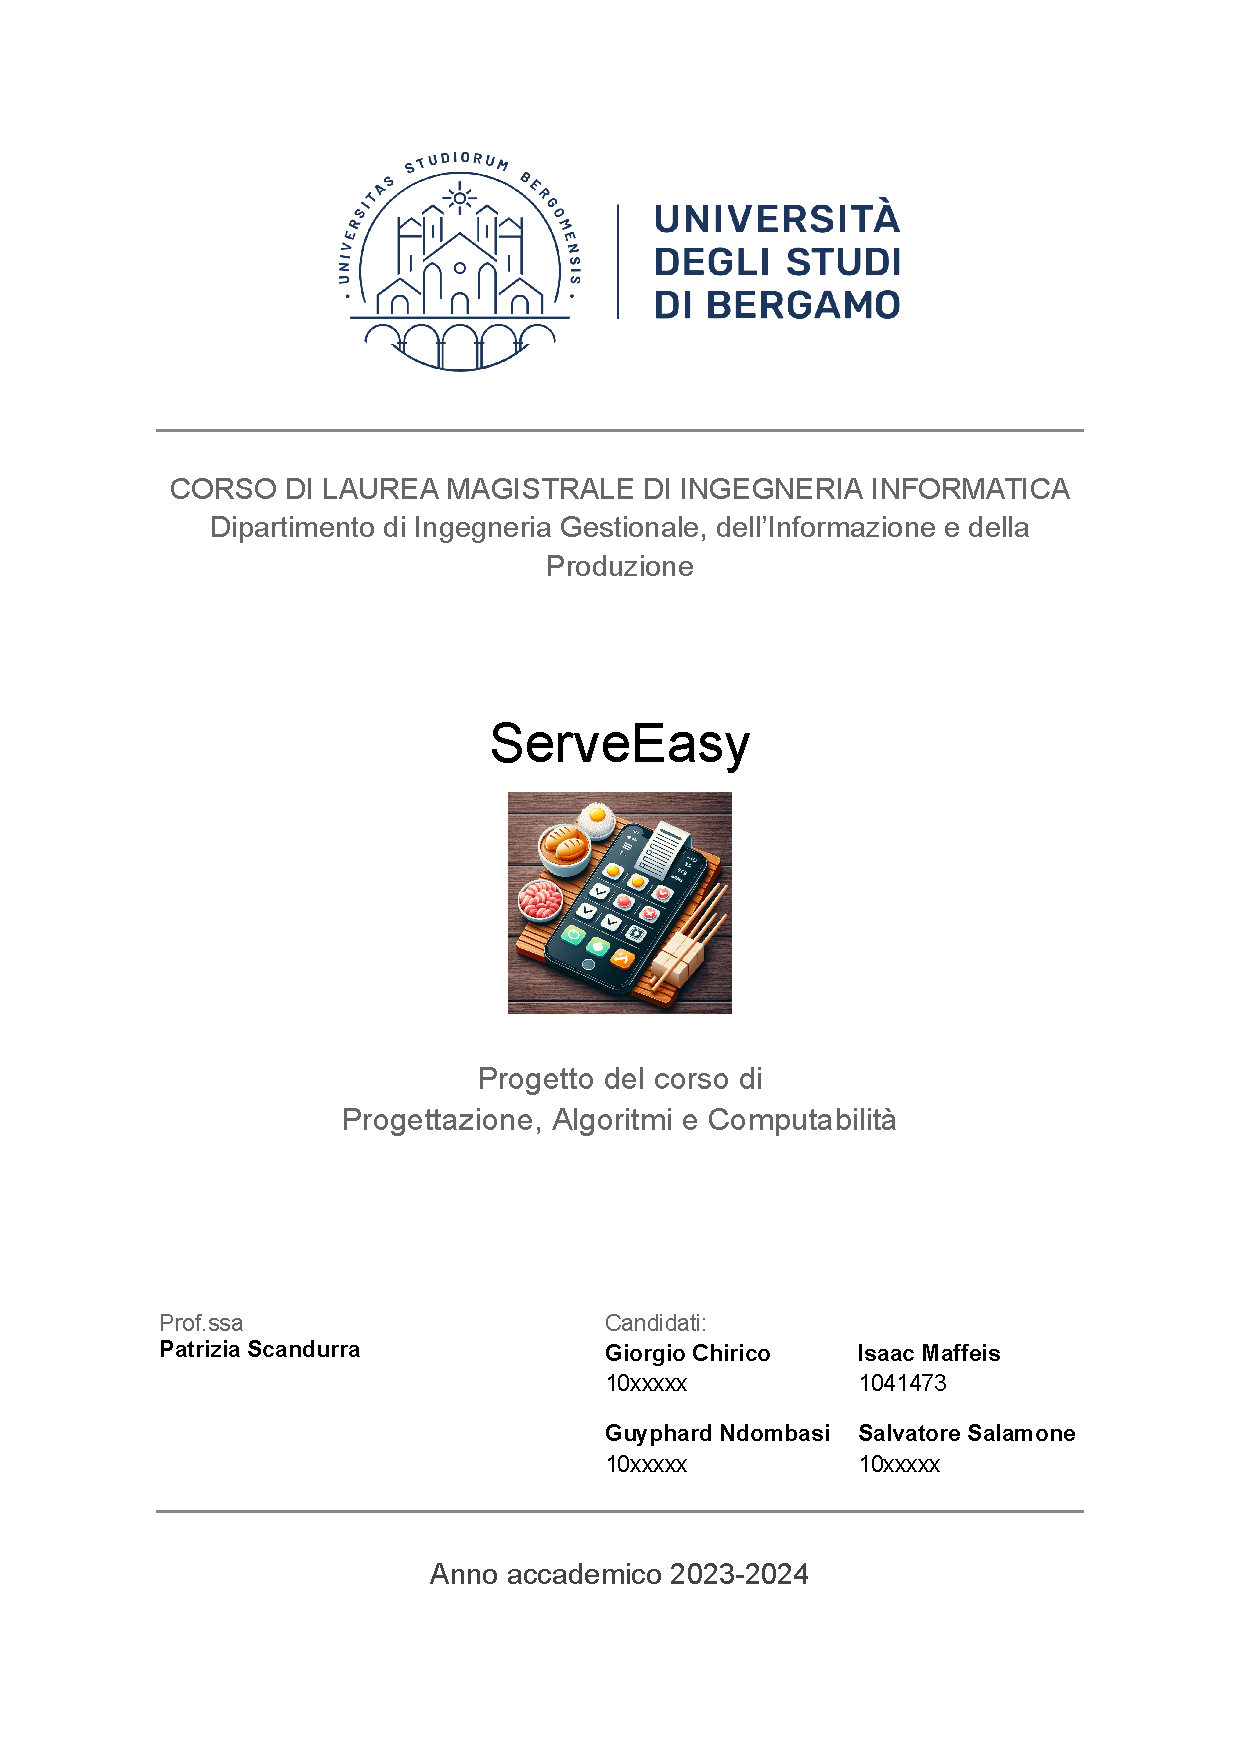
\includepdf[pages={1,{}},pagecommand={\thispagestyle{empty}}]{resources/Frontespizio.pdf}
%	\input{inizio/sommario}
	\mainmatter				
	\tableofcontents	% indice generale
	\listoffigures		% indice delle figure
	\lstlistoflistings  %indice del codice
	%	\addcontentsline{toc}{chapter}{Elenco dei codici}
	\chapter{Iterazione 0}
	\section{Introduzione}
Il sistema che si intende realizzare per il caso di studio è un software gestionale per ottimizzare la gestione delle comande di un ristorante, migliorando l’esperienza dei clienti, la produttività della cucina e l’efficacia della cassa.
Il sistema si baserà sull’utilizzo di tablet, che permettono ai commensali di ordinare i piatti desiderati, inserendo eventuali note, visualizzando lo stato degli ordini e richiedere il conto in modo semplice e veloce.
La cucina riceve le comande tramite una dashboard dedicata, che le ordina secondo un algoritmo di priorità basato su diversi parametri, come il tempo trascorso dall'ordinazione, la volontà del cliente, la durata di preparazione del piatto e altri fattori. La cucina può anche notificare il completamento di un ordine, che verrà visualizzato sul tablet del tavolo corrispondente. 
L’operatore di cassa sarà in grado di visualizzare il sommario degli ordini e stampare a schermo una ricevuta al cliente.
L'amministratore del ristorante può personalizzare la configurazione delle sale e dei menu, registrare i tavoli e gli account, e visualizzare delle statistiche sulle ordinazioni effettuate. Il sistema offre anche delle funzionalità opzionali, come la possibilità di far arrivare i piatti tutti insieme al tavolo, di allegare note agli ordini in preparazione, chiedere il conto al tavolo.
Il sistema si propone quindi di rendere più agile e soddisfacente il servizio di ristorazione, sfruttando le potenzialità della tecnologia e gli alti rendimenti di un algoritmo apposito.
\clearpage
	\section{Requisiti funzionali}
I requisiti funzionali sono stati esplicitati mediante il diagramma UML dei casi d’uso in \figurename~\ref{fig:use_cases_diagram}, il quale è composto da 4 attori (Amministratore, Cucina, Cassiere e Cliente che tramite ereditarietà viene ridefinito in Cliente al tavolo oppure Cliente che effettua ordinazioni d’asporto) e 6 viste (vista amministratore, vista cucina, vista cassiere, vista cliente, vista cliente al tavolo e sistema).

\begin{figure}[htbp]
	\begin{comment}
	The [htbp] option in LaTeX is used to fine-tune the placement of tables and figures.
	Each letter in [htbp] stands for a particular placement option:
	h (here): Place the table or figure in the text where the environment (like figure or table) is written, if there is enough room left on the page.
	t (top): Place it at the top of a page.
	b (bottom): Place it at the bottom of a page.
	p (page): Place it on a page containing only floats, such as figures and tables	
	LaTeX will try to place the float at the location that comes first in the option list.
	If it can’t place it there due to constraints like page size, it will move on to the next option. If none of the specified options work, LaTeX will hold the float until it finds a place where it fits, or until a \clearpage command is encountered
	\end{comment}
	\centering
	
	% verticale
	%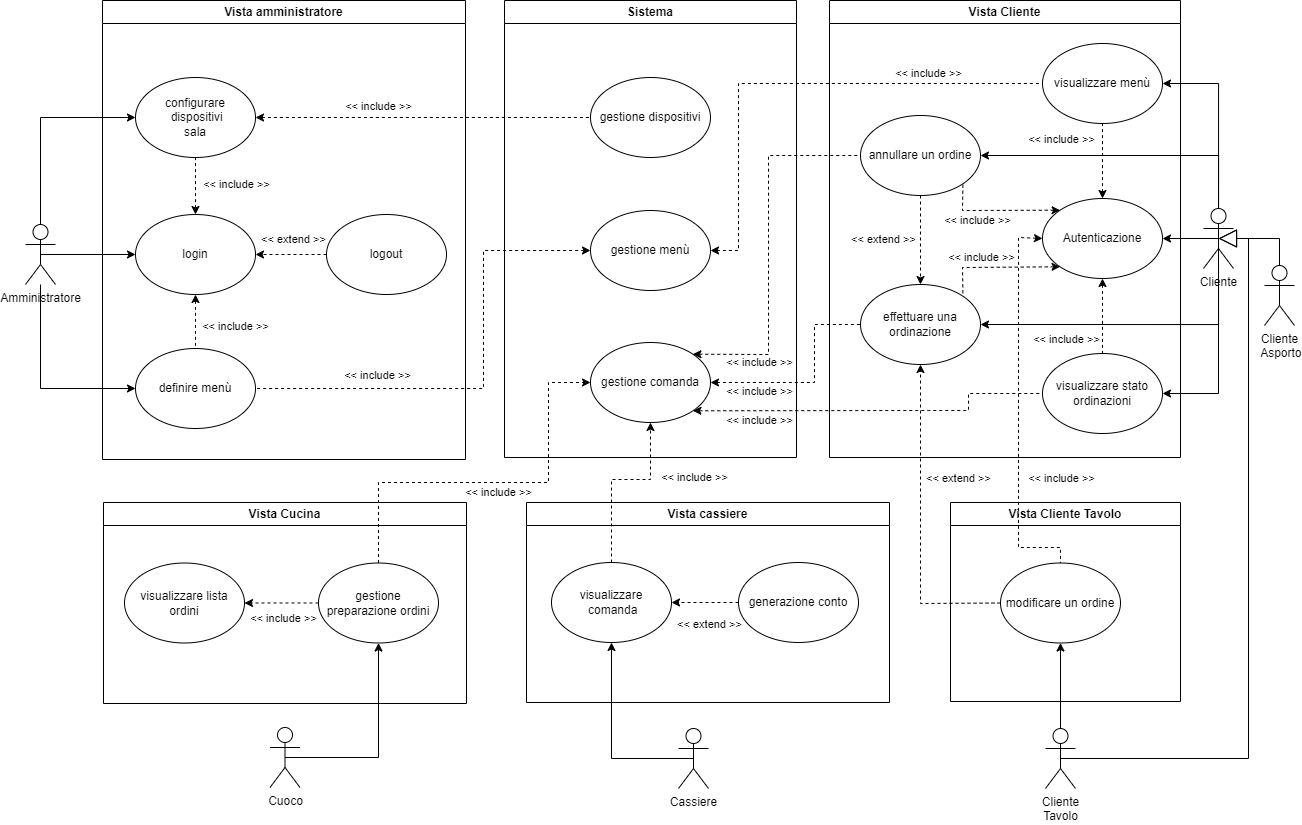
\includegraphics[scale=0.4, angle=90]{iterazione0/images/use_cases_diagram}
	
	% orizzontale
	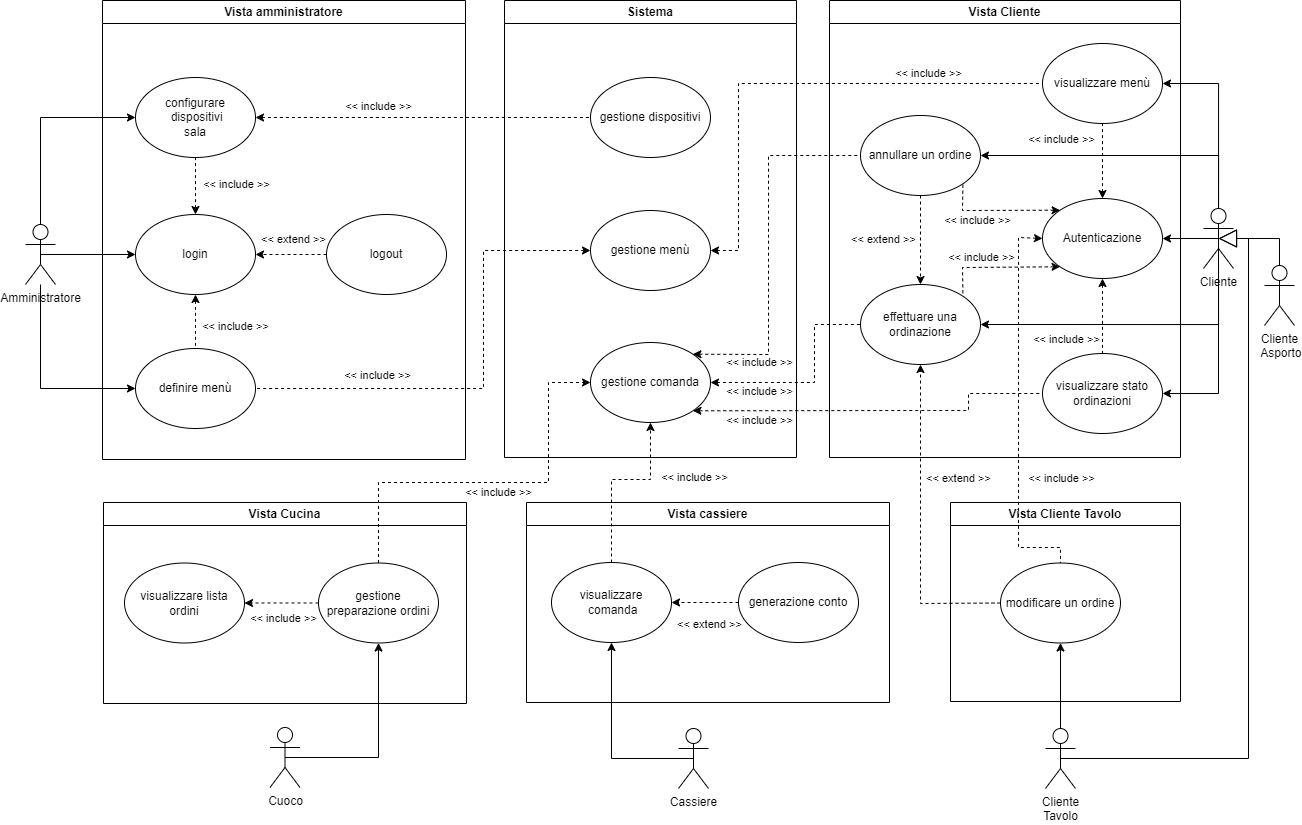
\includegraphics[scale=0.25]{iterazione0/images/use_cases_diagram}
	\caption{Diagramma dei casi d'uso\label{fig:use_cases_diagram}}
\end{figure}


Per ottimizzare il processo di sviluppo, si è deciso di categorizzare le specifiche funzionali in tabelle con tre livelli di priorità: elevata, media e bassa. Nello specifico il primo livello è assegnato alla Tabella~\ref{tab:use_cases_high_priority} a cui sono attribuiti i casi d'uso essenziali per il funzionamento dell'applicazione, i casi d'uso relativi alle funzionalità aggiuntive non critiche sono stati attribuiti alla Tabella~\ref{tab:use_cases_medium_priority} a priorità media, mentre il livello a bassa priorità che accoglie requisiti funzionali opzionali previsti per versioni successive alla Tabella~\ref{tab:use_cases_low_priority} .

\clearpage
\subsection{Priorità elevata}

\begin{table}[htbp]
	\centering
	 \begin{tabularx}{\textwidth}{|>{\centering\arraybackslash} m{4em}| >{\raggedright\arraybackslash}X |}
		\hline
		\textbf{Codice} & \textbf{Titolo} \\ [0.5ex]
		\hline\hline
		UC1 & Registrazione amministratore  \\
		\hline
		UC2 & Configurazione e gestione dispositivi (tavoli, cucina, cassa) \\
		\hline
		UC3 & Login/logout amministratore \\
		\hline
		UC4 & Gestione menù \\
		\hline
		UC5 & Algoritmo gestione coda ordini \\
		\hline
		UC6 & Cucina visualizza ordini da preparare \\
		\hline
		UC7 & Cucina notifica preparazione piatto \\
		\hline
		UC8 & Identificazione cliente \\
		\hline
		UC9 & Cliente visualizza menu \\
		\hline
		UC10 & Cliente effettua ordinazione \\
		\hline
		UC11 & Gestione sessione cliente \\
		\hline
		UC12 & Cassiere visualizza il conto \\
		\hline
	\end{tabularx}
	\caption{Casi d'uso ad elevata priorità}
	\label{tab:use_cases_high_priority}
\end{table}

\subsection{Priorità media}
\begin{table}[htbp]
	\centering
	\begin{tabularx}{\textwidth}{|>{\centering\arraybackslash} m{4em}| >{\raggedright\arraybackslash}X |}
		\hline
		\textbf{Codice} & \textbf{Titolo} \\ [0.5ex]
		\hline\hline
		UC13 & Modifica ordine al tavolo  \\
		\hline
		UC14 & Annullare un ordine \\
		\hline
		UC15 & Modifica priorità piatto (aumentare, diminuire) \\
		\hline
		UC16 & Cliente visualizza stato delle ordinazioni  \\
		\hline
	\end{tabularx}
	\caption{Casi d'uso a media priorità}
	\label{tab:use_cases_medium_priority}
\end{table}

\subsection{Priorità bassa}
\begin{table}[htbp]
	\centering
	\begin{tabularx}{\textwidth}{|>{\centering\arraybackslash} m{4em}| >{\raggedright\arraybackslash}X |}
		\hline
		\textbf{Codice} & \textbf{Titolo} \\ [0.5ex]
		\hline\hline
		UC17 & Identificazione cliente asporto  \\
		\hline
		UC18 & Cliente effettua ordinazione asporto  \\
		\hline
		UC19 & Gestione prioritaria ordinazioni da asporto \\
		\hline
		UC20 & Strategia greedy “a gruppi” (ingrediente principale in comune)   \\
		\hline
	\end{tabularx}
	\caption{Casi d'uso a bassa priorità}
	\label{tab:use_cases_low_priority}
\end{table}

\clearpage
	\section{Requisiti non funzionali}
Il progetto verrà sviluppato tenendo considerazione delle performance, integrabilità, modificabilità, testabilità e sicurezza dei componenti.

\subsection{Performance}
L'algoritmo di priorità impiegato dalla cucina per la selezione degli ordini deve fornire risultati in un tempo utile. Allo stesso tempo, gli utenti dell'applicativo web devono poter accedere e aggiornare le informazioni in un tempo accettabile.

\subsection{Integrabilità}
Ogni componente di sistema deve collaborare con gli altri componenti in modo da garantire le funzionalità previste dal sistema. Questa caratteristica è essenziale per garantire il corretto funzionamento e la coerenza dell'intero sistema.

\subsection{Modificabilità}
Il software deve facilitare l’aggiunta di nuovi componenti e funzionalità.

\subsection{Testabilità}
Ogni componente deve poter permettere la progettazione, implementazione ed esecuzione di test efficaci, in modo da garantire una massima copertura di requisiti e funzionalità.

\subsection{Sicurezza}
Il sistema deve integrare meccanismi di autenticazione ed autorizzazione degli attori, in modo da garantire la gestione delle identità, oltre alla protezione dei dati e delle API da accessi non autorizzati. Risulta dunque necessaria una distinzione dei ruoli con cui gli attori accedono al sistema.

\clearpage
	\section{Topologia}
Per il progetto è stata adottata una topologia three-tier al fine di separare in tre livelli distinti la presentazione dei dati, la gestione dell’applicativo e la mappatura dei dati sui dispositivi di archiviazione. Come si può vedere dalla \figurename~\ref{fig:topologia} il servizio è esposto tramite un web server, al quale i dispositivi clienti accedono, tramite richiesta HTTP/REST, per mezzo di una API unificata, con funzionalità di gateway. Il web-server usufruirà di database relazionali per lo storage (Data Layer), mentre sarà supportato da un database in-memory H2 (Application Layer) per avvantaggiarsi di una ridondanza dati, allo scopo di aumentare le performance lato client.

\begin{figure}[htbp]
	\centering
	
	% orizzontale
	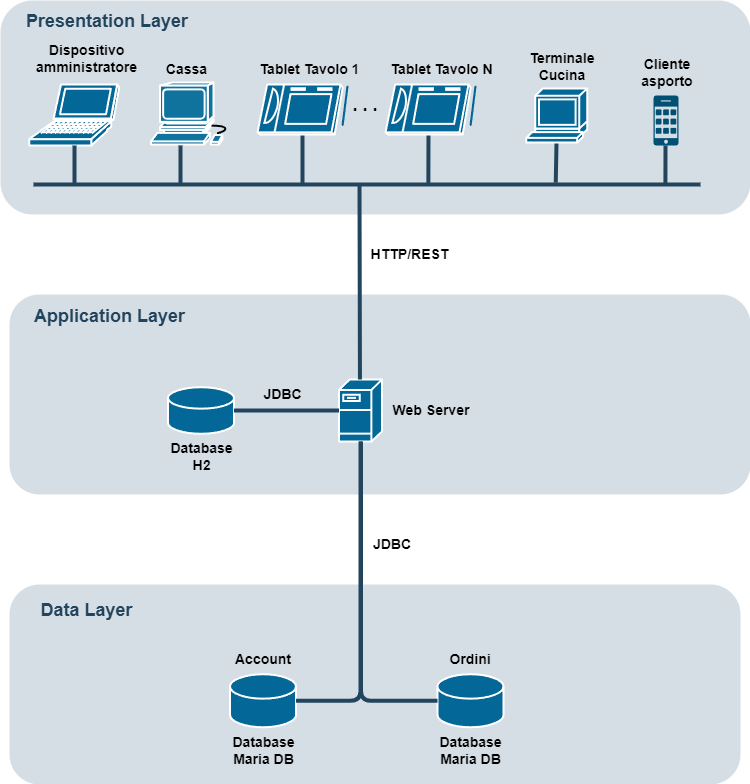
\includegraphics[scale=0.5]{iterazione0/images/topologia}
	\caption{Topologia del sistema\label{fig:topologia}}
\end{figure}

\clearpage
	\section{Toolchain}
Di seguito è presentata la toolchain utilizzata per lo sviluppo del progetto software
\subsection{Modellazione}
\begin{itemize}
	\item draw.io: casi d’uso e topologia;
\end{itemize}

\subsection{Stack applicativo}
\begin{itemize}
	\item Angular.js: front-end;
	\item Java Spring Boot 3.x.x: back-end;
	\item MariaDB: database per l’archiviazione;
	\item H2: database in-memory per rendere più efficiente l’estrazione dei dati;
\end{itemize}

\subsection{Deployment}
\begin{itemize}
	\item Docker: piattaforma per container virtuali;
	\item Docker Compose: gestione app multi-container;
\end{itemize}

\subsection{Gestore repository}
\begin{itemize}
	\item Git: Controllo versione per codice sorgente;
	\item GitHub: Piattaforma hosting e collaborativa per progetti Git;
\end{itemize}

\subsection{Continuous Integration}
\begin{itemize}
	\item Maven: gestore di progetti e dipendenze Java;
	\item GitHub Action: piattaforma di automazione per repository GitHub;
	\item Jenkins: strumento di automazione per sviluppatori;
\end{itemize}

\subsection{Analisi statica}
\begin{itemize}
	\item CodeMR su JetBrains: visualizzazione di alto livello di metriche qualitative del codice;
\end{itemize}

\subsection{Analisi dinamica}
\begin{itemize}
	\item Postman: strumento per testare API e servizi;
	\item Garfana: analisi delle performance della rete di microservizi;
	\item JUNIT: framework per test unitari Java;
\end{itemize}

\subsection{Documentazione e organizzazione del team}
\begin{itemize}
	\item Google Drive: servizio cloud per archiviazione;
	\item Documenti condivisi di Google: per elaborare la documentazione in modo condiviso;
	\item \LaTeX: generazione documentazione;
	\item Microsoft Teams: per organizzazione e meeting;
\end{itemize}

\subsection{Modello di sviluppo}
Il modello adottato segue la filosofia AGILE, con enfasi sui seguenti aspetti-chiave:
\begin{itemize}
	\item pair programming, per favorire creatività e controllo del lavoro prodotto;
	\item orientamento al risultato, con enfasi maggiore sulla generazione di codice funzionante e componenti completi prima della relativa documentazione;
	\item rapidità di risposta ai cambiamenti;
	\item collaborazione attiva col cliente, al fine di incontrare le sue necessità, garantire trasparenza e fornire feedback tempestivo sul lavoro di progetto;
	\item Proattività nell’identificazione e mitigazione dei rischi.
\end{itemize}

\clearpage
	\chapter{Iterazione 1}
	\section{Introduzione}
Il sistema che si intende realizzare per il caso di studio è un software gestionale per ottimizzare la gestione delle comande di un ristorante, migliorando l’esperienza dei clienti, la produttività della cucina e l’efficacia della cassa.
Il sistema si baserà sull’utilizzo di tablet, che permettono ai commensali di ordinare i piatti desiderati, inserendo eventuali note, visualizzando lo stato degli ordini e richiedere il conto in modo semplice e veloce.
La cucina riceve le comande tramite una dashboard dedicata, che le ordina secondo un algoritmo di priorità basato su diversi parametri, come il tempo trascorso dall'ordinazione, la volontà del cliente, la durata di preparazione del piatto e altri fattori. La cucina può anche notificare il completamento di un ordine, che verrà visualizzato sul tablet del tavolo corrispondente. 
L’operatore di cassa sarà in grado di visualizzare il sommario degli ordini e stampare a schermo una ricevuta al cliente.
L'amministratore del ristorante può personalizzare la configurazione delle sale e dei menu, registrare i tavoli e gli account, e visualizzare delle statistiche sulle ordinazioni effettuate. Il sistema offre anche delle funzionalità opzionali, come la possibilità di far arrivare i piatti tutti insieme al tavolo, di allegare note agli ordini in preparazione, chiedere il conto al tavolo.
Il sistema si propone quindi di rendere più agile e soddisfacente il servizio di ristorazione, sfruttando le potenzialità della tecnologia e gli alti rendimenti di un algoritmo apposito.
\clearpage
	\section{Use Cases}

Si sono presi in considerazione i seguenti casi d'uso, ossia quelli a priorità più elevata della Tabella~\ref{tab:use_cases_high_priority}

\begin{table}[htbp]
	\centering
	\begin{tabularx}{\textwidth}{|>{\centering\arraybackslash} m{4em}| >{\raggedright\arraybackslash}X |}
		\hline
		\textbf{Codice} & \textbf{Titolo} \\ [0.5ex]
		\hline\hline
		UC1 & Gestione comanda  \\
		\hline
		UC2 & Effettuare un'ordinazione \\
		\hline
		UC3 & Visualizzare menù \\
		\hline
		UC4 & Autenticazione \\
		\hline
		UC5 & Visualizzare lista ordini \\
		\hline
		UC6 & Gestione preparazione ordini \\
		\hline
	\end{tabularx}
	\caption{Casi d'uso presi in considerazione nell'iterazione 1}
	\label{tab:use_cases_it1}
\end{table}

\begin{figure}[htbp]
	\centering
	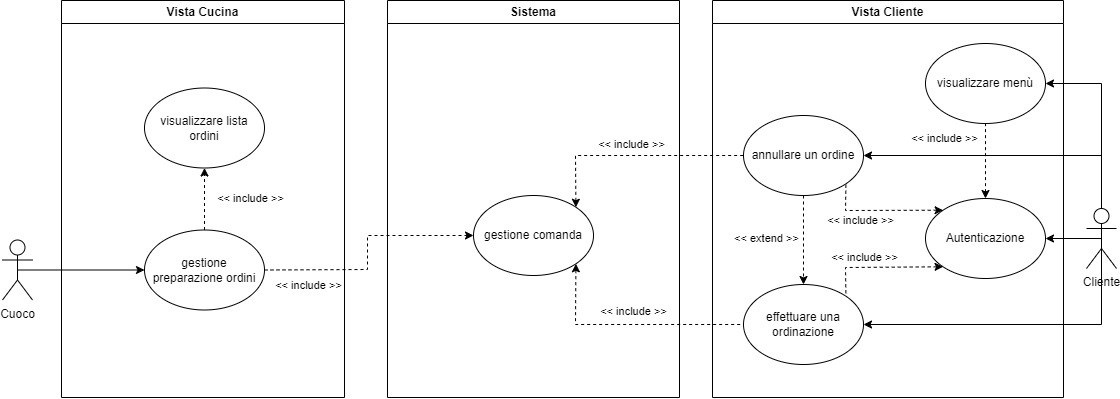
\includegraphics[scale=0.36]{iterazione1/images/useCases_it1.jpg}
	\caption{Casi d'uso presi in considerazione nell'iterazione 1\label{fig:use_cases_it1}}
\end{figure}

Per facilitare una migliore organizzazione e comprensione del sistema, i casi d'uso vengono raggruppati nel seguente modo:

\subsection{Gruppo Sistema}
\paragraph{UC-1 “Gestione Comanda”:}
\begin{itemize}
	\item UC-1.1 : gestione priorità ordine \\ ogni ordine è caratterizzato da una priorità
	\item UC-1.2 : gestione coda ordini \\
	ogni ordine è inserito in una coda ordini
	\item UC-1.3 : assegnazione ordini comanda \\
	ogni ordine deve essere associato ad una comanda
	\item UC-1.4 : assegnazione comanda cliente \\
	ogni comanda deve essere associata ad un cliente
\end{itemize}

\subsection{Gruppo cliente}
\paragraph{UC-2 “effettuare un’ordinazione”:}
\begin{itemize}
	\item UC-2.1 : effettuare un ordine personalizzato \\
	il cliente può effettuare un ordine escludendo un ingrediente o descrivendo una variazione del piatto
\end{itemize}

\paragraph{UC-3 “Visualizzare menu”:}
\begin{itemize}
	\item UC-3.1 : visualizzare piatto 
	\item UC-3.2 : visualizzare informazioni piatto \\
	il cliente deve poter leggere breve descrizione, ingredienti, prezzo
\end{itemize}

\paragraph{UC-4 “Autenticazione”:}
\begin{itemize}
	\item UC-4.1 : identificazione sessione cliente \\ 
	al momento del pasto e solo per il pasto, il cliente deve poter distinguere la propria comanda
\end{itemize}

\subsection{Gruppo cuoco}
\paragraph{UC-5 “visualizzare lista ordini”:}
\begin{itemize}
	\item UC-5.1 : visualizzazione ordini per postazione \\ 
	il cuoco deve visualizzare gli ordini destinati alla sua postazione
\end{itemize}

\paragraph{UC-6 “gestione preparazione ordini”:}
\begin{itemize}
	\item UC-6.1 : notifica preparazione ordine \\ 
	il cuoco deve segnalare la presa in carico dell’ordine
	\item UC-6.2 : notifica completamento ordine \\
	il cuoco deve segnalare il completamento dell’ordine così da passare al successivo
	\item UC-6.3 : gestione priorità postazione \\
	il cuoco può modificare la priorità di un certo ingrediente così da ridurre la pressione su una certa postazione o, viceversa, per aumentarne il traffico. In tal modo può manualmente agire sulla gestione del traffico verso la cucina.
\end{itemize}

\clearpage
	\section{Component Diagram}
\subsection{Sistema ServeEasy}
\subsubsection{single component del sistema}
\begin{figure}[H]
	\centering
	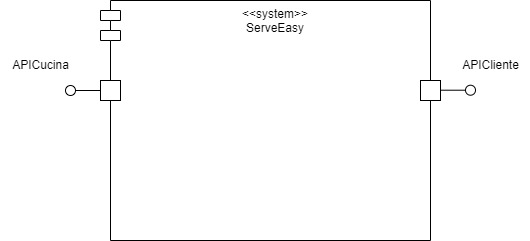
\includegraphics[scale=0.6]{iterazione1/images/ServeEasy_componente_unico.jpg}
	\caption{Component diagram - ServeEasy\label{fig:component_diagram_serveeasy}}
\end{figure}
Visualizzazione iniziale della soluzione come un componente unico che espone due API, dedicate rispettivamente alla cucina ed ai clienti. Si procede con uno sviluppo top-down.

\subsubsection{primo zoom-in sul sistema}

\begin{figure}[H]
	\centering
	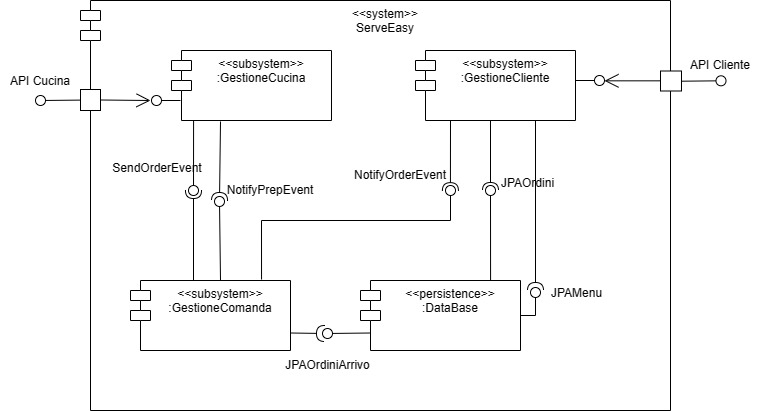
\includegraphics[scale=0.5]{iterazione1/images/ServeEasy_primo_zoomin.jpg}
	\caption{Component diagram - System\label{fig:component_diagram_system}}
\end{figure}
Al primo zoom-in si identificano i servizi che andranno a comporre l’architettura della soluzione:
\begin{itemize}
	\item \textbf{GestioneComanda:} risolve gli use case del gruppo “sistema”, rappresenta il cuore del sistema ed incorpora la logica di backend fondamentale per la gestione regolarizzata degli ordini da cliente a cucina, attraverso politiche di schedulazione a priorità progettate ed implementate con un algoritmo ad-hoc.
	\item \textbf{GestioneCliente:} risolve gli use case del gruppo “cliente”, espone le funzionalità destinate ai dispositivi di tavolo ed al portale web per clienti d’asporto. Ha dunque il compito di gestire gli aspetti del servizio legati alle interazioni del cliente col sistema, come la visualizzazione del menu, la creazione degli ordini ed il raggruppamento degli ordini in una comanda relativa.
	\item \textbf{GestioneCucina:} risolve gli use case del gruppo “cucina”, espone le chiamate destinate ai dispositivi di cucina. Questo servizio conterrà un sistema a code, dove l’ordine in arrivo verrà classificato ed inserito in base al suo ingrediente principale. Gli ordini verranno gestiti dalle postazioni della cucina seguendo una politica FIFO.
\end{itemize}
Per la memorizzazione persistente dei dati cruciali per l’attività come piatti, ordini e comande, è stato inserito un componente database.
All’interno del sistema ServeEasy, i componenti comunicano tra loro attraverso una comunicazione ad eventi, asincrona. Si è deciso di attuare una politica pub-sub per la gestione delle comunicazioni interne, costituite da scambi di notifiche e DTO tra i microservizi designati.

\subsection{Gestione Comanda}
\subsubsection{Componenti esagonali}
Il design dei microservizi seguirà l’architettura esagonale: un dominio, denominato “Domain”, nucleo della logica di servizio, sarà racchiuso tra due gusci denominati “Interface” e “Infrastructure”, i quali avranno il compito di astrarre la gestione dati, rendendola opaca al dominio. La logica di base del microservizio seguirà lo schema port-adapter, dove il dominio comunica con i gusci attraverso delle interfacce dette porte (il cui nome nel progetto è caratterizzato dal suffisso “Port”), mentre i gusci hanno il compito di implementare l’effettivo componente di trasmissione (guscio Infrastructure) e/o ricezione (guscio Interface), detto adattatore (sarà identificabile da suffisso “Adapter”). 
Nello specifico il \textbf{Domain} definisce gli oggetti, le entità e le operazioni che sono pertinenti al problema che il microservizio gestisce.Gli \textbf{Interface adapters} fungono da ponte tra il mondo esterno e il core del sistema, consentendo al microservizio di comunicare con altre applicazioni, servizi o dispositivi esterni in modo indipendente dall'implementazione interna del sistema stesso, mentre gli \textbf{Infrastructure adapters} fungono da ponte tra il core del sistema e l'infrastruttura esterna, gestendo le chiamate e le operazioni necessarie per accedere e utilizzare le risorse infrastrutturali.
Tali caratteristiche avvantaggiano l’intercambiabilità dei singoli componenti di sistema a costo di un aumento della complessità.
\begin{figure}[H]
	\centering
	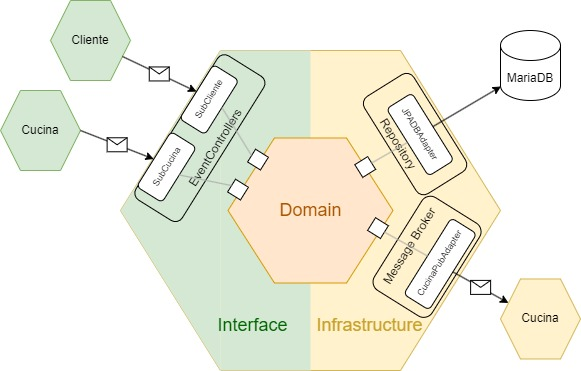
\includegraphics[scale=0.7]{iterazione1/images/hexagon.jpg}
	\caption{Architettura esagonale per il microservizio Gestione comanda\label{fig:hexagon}}
\end{figure}

\subsubsection{zoom-in gestione comanda}
\begin{figure}[H]
	\centering
	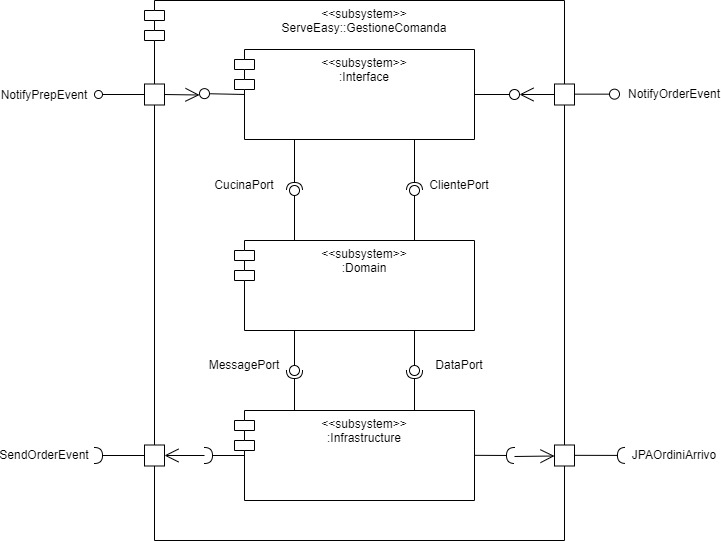
\includegraphics[scale=0.5]{iterazione1/images/component_comanda_cucina-GestioneComanda.jpg}
	\caption{Component diagram - Gestione Comanda\label{fig:component_diagram_gestione_comanda}}
\end{figure}


\subsubsection{zoom-in infrastructure di gestione comanda}
\begin{figure}[H]
	\centering
	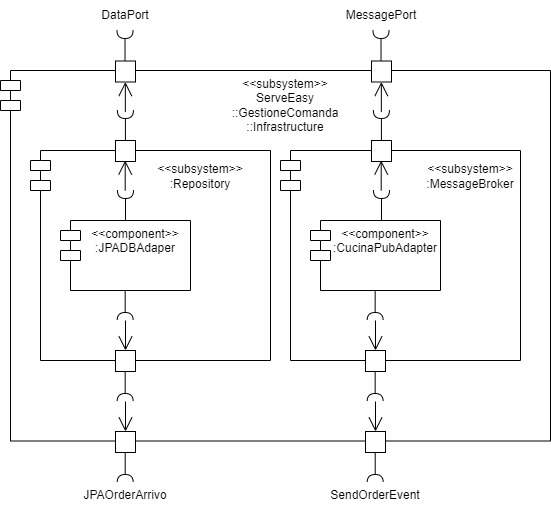
\includegraphics[scale=0.5]{iterazione1/images/component_comanda_cucina-GestioneComanda__Infrastructure.jpg}
	\caption{Component diagram - Gestione Comanda - Infrasrtructure \label{fig:component_diagram_gestione_comanda_infrastracture}}
\end{figure}

\subsubsection{zoom-in domain di gestione comanda}
\begin{figure}[H]
	\centering
	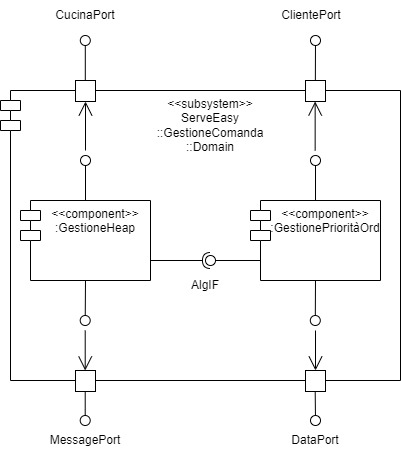
\includegraphics[scale=0.5]{iterazione1/images/component_comanda_cucina-GestioneComanda__Domain.jpg}
	\caption{Component diagram - Gestione Comanda - Domain \label{fig:component_diagram_gestione_comanda_domain}}
\end{figure}

\subsubsection{zoom-in interface di gestione comanda}
\begin{figure}[H]
	\centering
	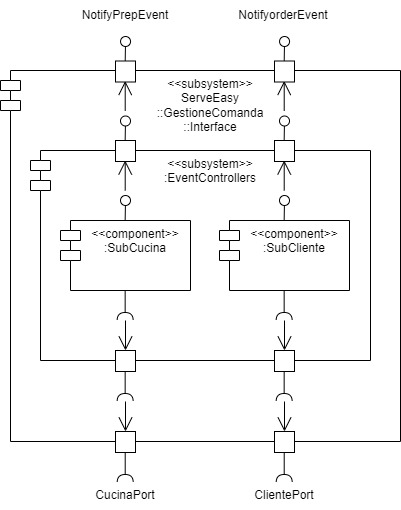
\includegraphics[scale=0.5]{iterazione1/images/component_comanda_cucina-GestioneComanda__Interface.jpg}
	\caption{Component diagram - Gestione Comanda - Interface \label{fig:component_diagram_gestione_comanda_interface}}
\end{figure}

\subsection{Gestione Cucina}
\subsubsection{zoom-in gestione cucina}
\begin{figure}[H]
	\centering
	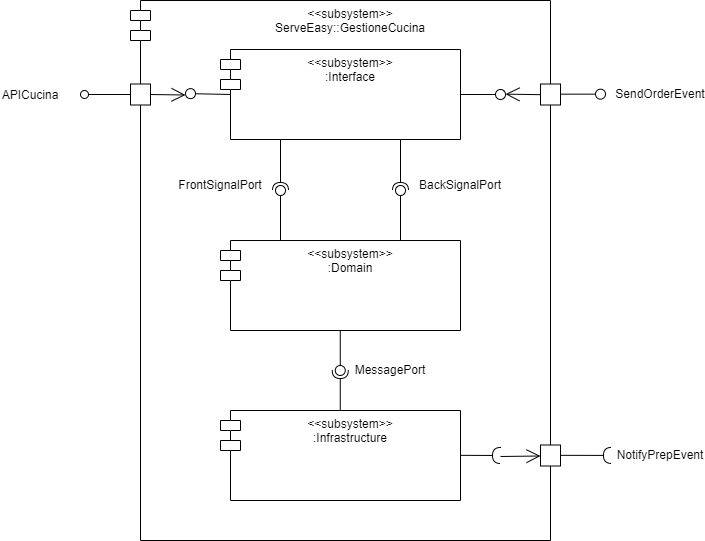
\includegraphics[scale=0.5]{iterazione1/images/component_comanda_cucina-GestioneCucina.jpg}
	\caption{Component diagram - Gestione Cucina \label{fig:component_diagram_gestione_cucina}}
\end{figure}

\subsubsection{zoom-in infrastructure di gestione cucina}
\begin{figure}[H]
	\centering
	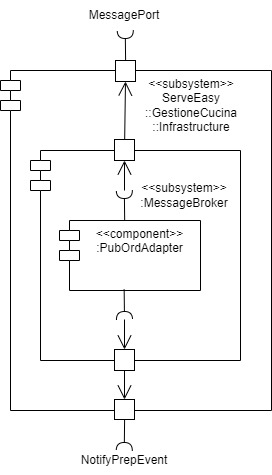
\includegraphics[scale=0.5]{iterazione1/images/component_comanda_cucina-GestioneCucina__Infrastructure.jpg}
	\caption{Component diagram - Gestione Cucina - Infrastructure \label{fig:component_diagram_gestione_cucina_infrastructure}}
\end{figure}

\subsubsection{zoom-in domain di gestione cucina}
\begin{figure}[H]
	\centering
	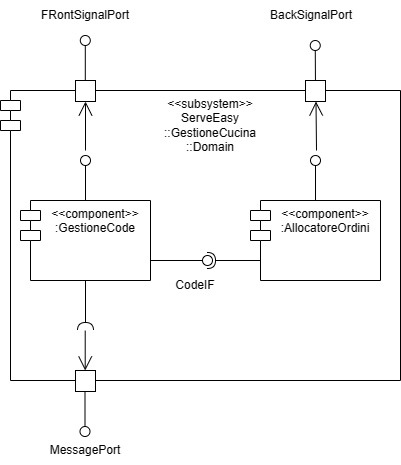
\includegraphics[scale=0.5]{iterazione1/images/component_comanda_cucina-GestioneCucina__Domain.jpg}
	\caption{Component diagram - Gestione Cucina - Domain \label{fig:component_diagram_gestione_cucina_domain}}
\end{figure}

\subsubsection{zoom-in interface di gestione cucina}
\begin{figure}[H]
	\centering
	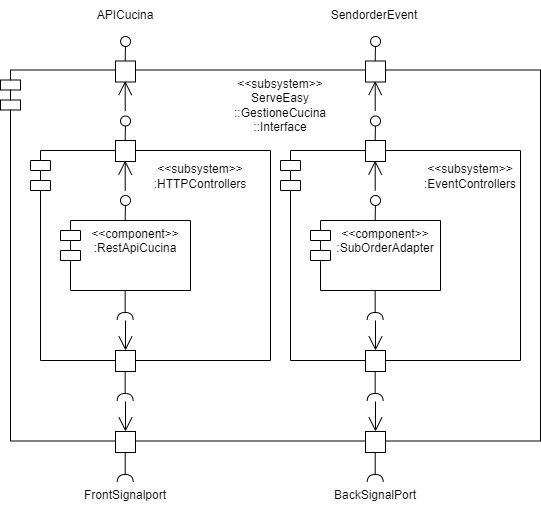
\includegraphics[scale=0.5]{iterazione1/images/component_comanda_cucina-GestioneCucina__Interface.jpg}
	\caption{Component diagram - Gestione Cucina - Interface \label{fig:component_diagram_gestione_cucina_interface}}
\end{figure}

\subsection{Gestione Cliente}
\subsubsection{zoom-in gestione cliente}
\begin{figure}[H]
	\centering
	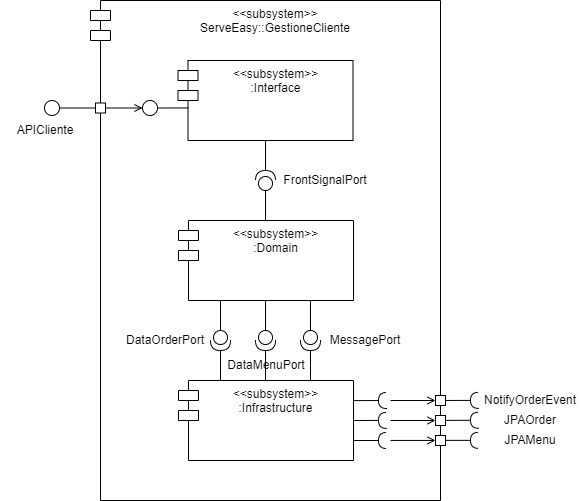
\includegraphics[scale=0.5]{iterazione1/images/GestioneCliente_subsystem-GestioneCliente.jpg}
	\caption{Component diagram - Gestione Cliente \label{fig:component_diagram_gestione_cliente}}
\end{figure}

\subsubsection{zoom-in infrastructure di gestione cliente}
\begin{figure}[H]
	\centering
	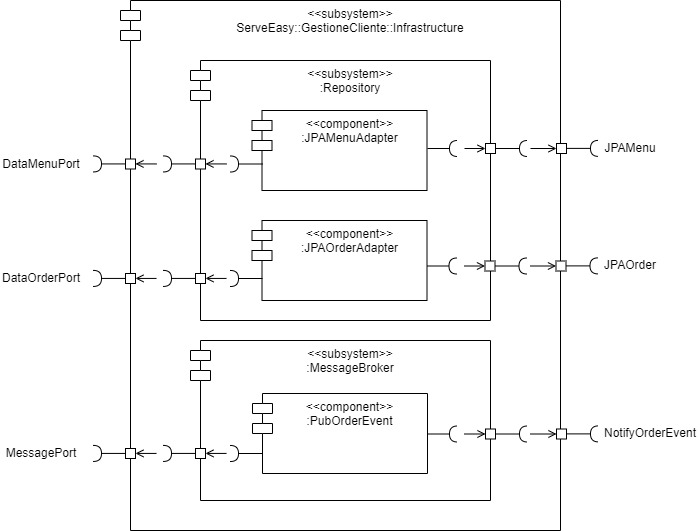
\includegraphics[scale=0.5]{iterazione1/images/GestioneCliente_subsystem-Infrastructure.jpg}
	\caption{Component diagram - Gestione Cliente - Infrastructure \label{fig:component_diagram_gestione_cliente_infrastructure}}
\end{figure}

\subsubsection{zoom-in domain di gestione cliente}
\begin{figure}[H]
	\centering
	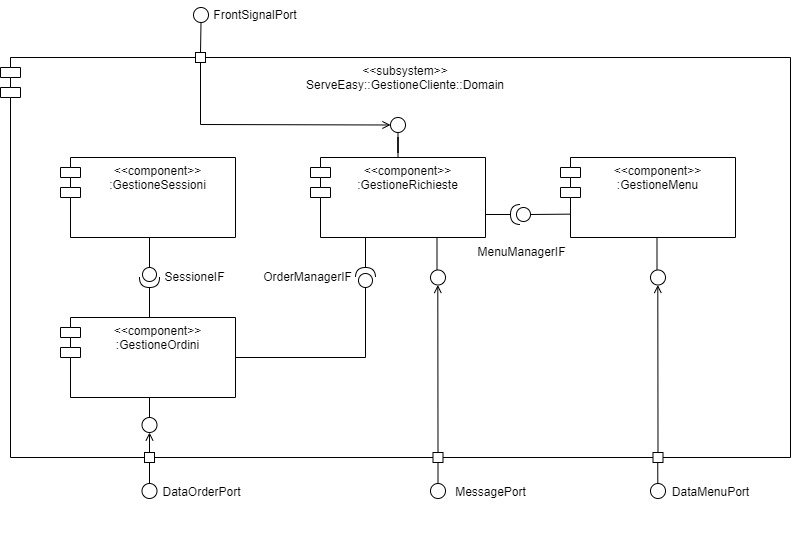
\includegraphics[scale=0.5]{iterazione1/images/GestioneCliente_subsystem-Domain.jpg}
	\caption{Component diagram - Gestione Cliente - Domain \label{fig:component_diagram_gestione_cliente_domain}}
\end{figure}

\subsubsection{zoom-in interface di gestione cliente}
\begin{figure}[H]
	\centering
	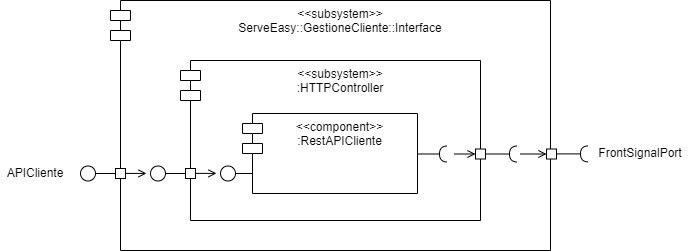
\includegraphics[scale=0.5]{iterazione1/images/GestioneCliente_subsystem-Interface.jpg}
	\caption{Component diagram - Gestione Cliente - Interface \label{fig:component_diagram_gestione_cliente_interface}}
\end{figure}

\clearpage
	\section{Database}
Per facilitare l'identificazione delle entità coinvolte nel database si è utilizzato un modello entità-relazione che fornisce una rappresentazione grafica chiara e intuitiva della struttura dei dati. Questo modello aiuta a visualizzare le entità (oggetti o concetti del mondo reale), le relazioni (le associazioni tra le entità) e gli attributi (le proprietà o le caratteristiche delle entità e delle relazioni).
\subsection{Modello Entità-Relazione}
Nel seguente diagramma entità-relazione in Figura~\ref{fig:er_diagram}, osserviamo che le comande possono essere costituite da più ordini effettuati dai clienti. Tali clienti sono suddivisi in due categorie: clienti d’asporto identificati tramite numero di telefono e clienti al tavolo identificati tramite numero del tavolo. I piatti, consultabili tramite un menù, sono caratterizzati da un ingrediente principale. Una volta ordinato un piatto dal menù, questo viene inserito al’interno di un ordine identificato da un codice progressivo per cliente, e viene successivamente inserito nella comanda del rispettivo cliente. La comanda sarà quindi utilizzata per identificare il cliente e contiene i piatti ordinati oltre che il totale dello scontrino con il corrispettivo codice di pagamento.

\begin{figure}[H]
	\centering
	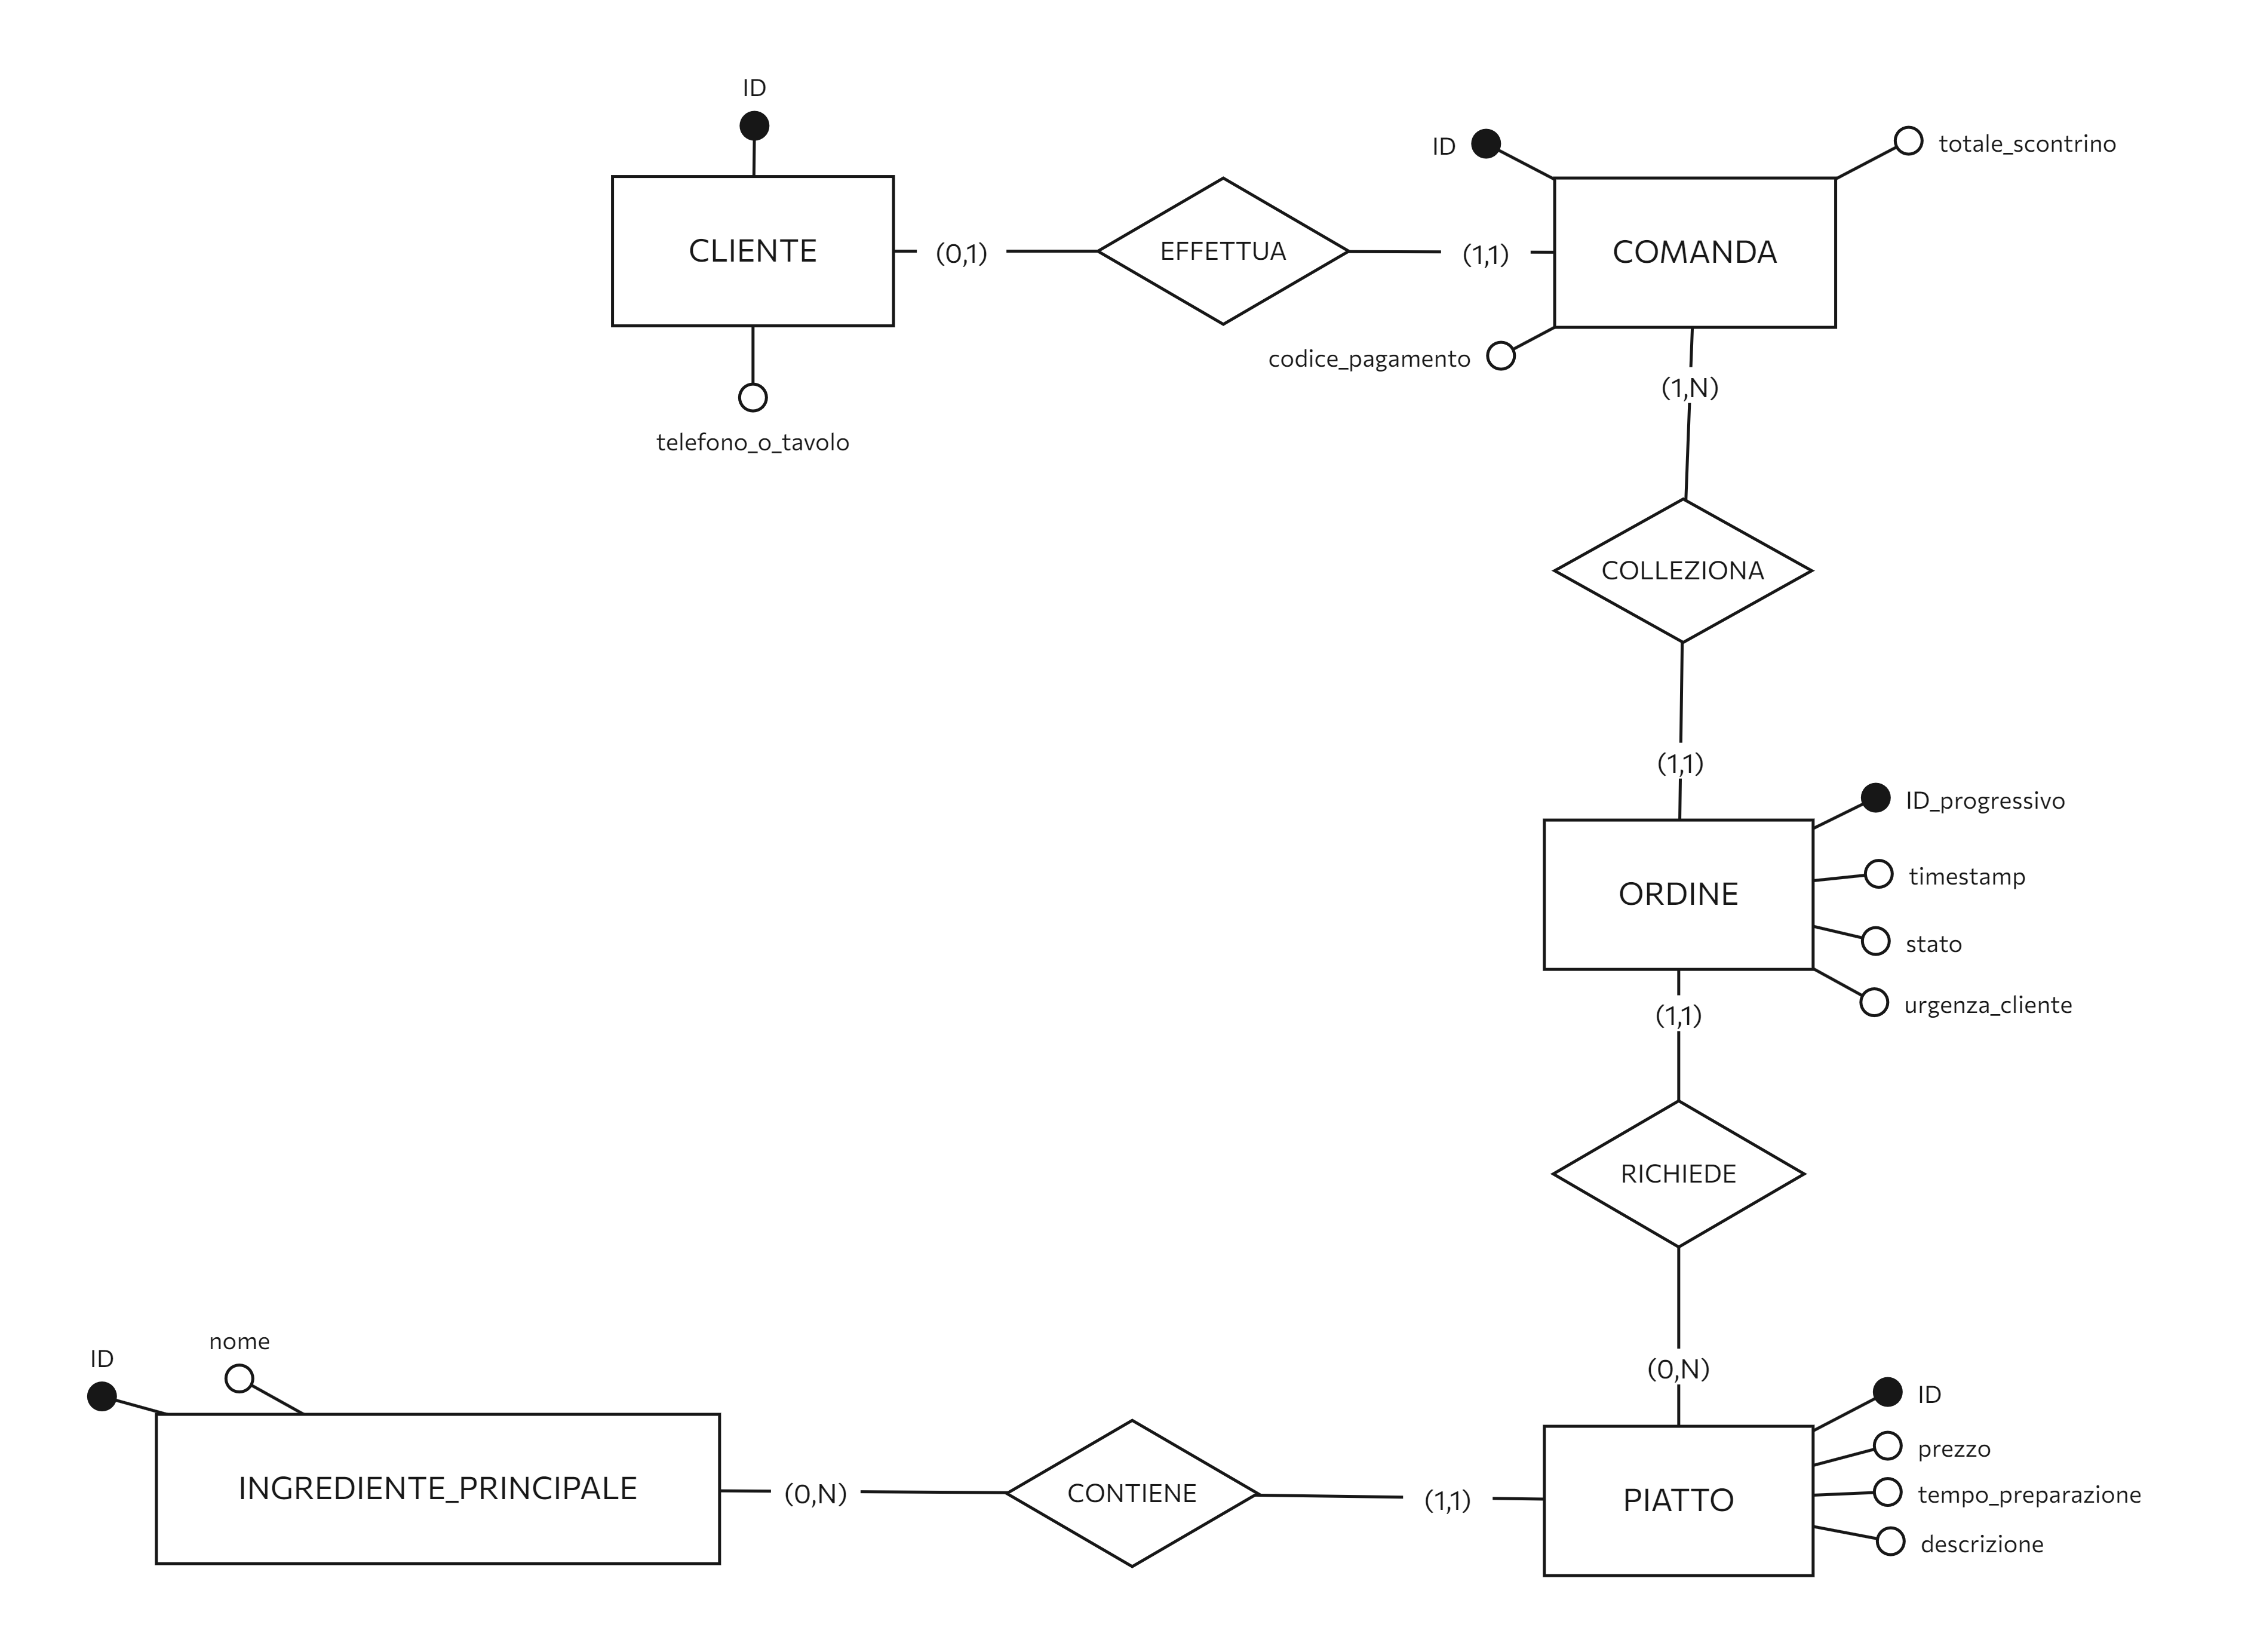
\includegraphics[scale=0.4]{iterazione1/images/ER_project_c.png}
	\caption{Modello Entità-relazione\label{fig:er_diagram}}
\end{figure}

\subsection{Modello logico}
Tramite il modello logico viene rappresentata in modo astratto la struttura dei dati così da facilitare la progettazione del database, definendo come i dati sono organizzati e come le entità interagiscono tra loro.
Rappresentazione della struttura dei dati all’interno del database. L’attributo di cliente::asporto\_o\_tavolo è stato pensato come un boolean in quanto il cliente può essere di due tipi:
\begin{itemize}
	\item se asporto\_o\_tavolo = 0, allora l’ID sarà il codice identificativo di un tavolo;
	\item se asporto\_o\_tavolo = 1, allora l’ID sarà un numero di telefono;
\end{itemize}

\begin{figure}[htbp]
	\centering
	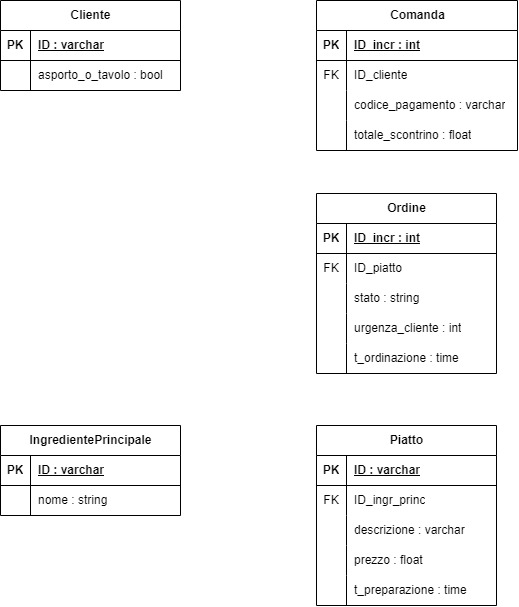
\includegraphics[scale=0.5]{iterazione1/images/database_modello_logico.jpg}
	\caption{Modello Logico\label{fig:modello_logico}}
\end{figure}

\newpage
Il modello logico è implementato con le seguenti query al database:

\begin{lstlisting}[language=SQL,caption=Query del database in SQL,label=lst:sqlcode]
	CREATE TABLE IF NOT EXISTS Cliente(
	ID varchar(10) PRIMARY KEY,
	t_o_a boolean NOT NULL
	);
	
	CREATE TABLE IF NOT EXISTS Comanda (
	ID int(10) AUTO_INCREMENT,
	ID_cliente varchar(10) NOT NULL,
	codice_pagamento varchar(255) DEFAULT NULL,
	totale_scontrino float DEFAULT 0.0,
	PRIMARY KEY (ID),
	FOREIGN KEY (ID_cliente) REFERENCES Cliente(ID)
	);
	
	CREATE TABLE IF NOT EXISTS IngredientePrincipale(
	ID varchar(20) PRIMARY KEY,
	nome varchar(20) NOT NULL
	);
	
	CREATE TABLE IF NOT EXISTS Piatto(
	ID varchar(20) NOT NULL PRIMARY KEY,
	ID_ingr_princ varchar(20) NOT NULL,
	descrizione varchar(50),
	prezzo float(6) NOT NULL,
	t_preparazione TIMESTAMP DEFAULT CURRENT_TIMESTAMP,
	FOREIGN KEY (ID_ingr_princ) REFERENCES IngredientePrincipale(ID)
	);
	
	CREATE TABLE IF NOT EXISTS Ordine(
	ID int(10) NOT NULL AUTO_INCREMENT,
	ID_comanda int(10) NOT NULL,
	ID_piatto varchar(20) NOT NULL,
	stato int(1) DEFAULT 0, -- 0=in preparazione, 1=completato
	t_ordinazione TIMESTAMP DEFAULT CURRENT_TIMESTAMP,
	urgenza_cliente int(2) DEFAULT 0, -- priorita' del cliente: 1=massima, -1=minima
	PRIMARY KEY (ID,ID_comanda),
	FOREIGN KEY (ID_comanda) REFERENCES Comanda(ID),
	FOREIGN KEY (ID_piatto) REFERENCES Piatto(ID),
	CHECK (stato >= 0 AND stato <=1 )
	);
\end{lstlisting}

\clearpage
	\section{Algoritmo}
\subsection{Briefing}
Nell'ambito di questa applicazione si considera che ogni piatto sia composto da un ingrediente principale e da più ingredienti secondari. 
Ogni piatto ordinato viene chiamato ordine, quindi un ordine comprende un singolo piatto, mentre la comanda contiene tutti gli ordini di un singolo cliente.
Nel corso di un brainstorming, si è maturata l’idea di organizzare la cucina in postazioni, ognuna focalizzata su un ingrediente principale: ogni postazione si occuperà quindi di preparare e completare piatti accomunati dallo stesso ingrediente principale.
\subsection{Organizzazione} 
Di seguito viene illustrata l’organizzazione delle entità coinvolte nella gestione dell’algoritmo:
\subsubsection{Ordine}
Ogni ordine contiene un singolo piatto del menù, viene classificato per ingrediente principale univoco (es. riso, pasta, pesce, …), ogni ordine presenta poi più parametri, questi contribuiscono a calcolare la priorità ad esso associata.
Parametri ordine:
\begin{itemize}
	\item Ingrediente principale;
	\item Tempo di preparazione;
	\item Numero ordine effettuato (primo, secondo, …);
	\item Urgenza del cliente;
	\item Tempo in attesa.
\end{itemize}

\subsubsection{Cucina}
La cucina viene organizzata in postazioni di lavoro, ossia delle aree dedicate organizzate per svolgere specifiche attività culinarie adibite alla preparazione di piatti che hanno in comune il medesimo ingrediente principale, nello specifico:
\begin{itemize}
	\item ogni postazione di lavoro è adibita al massimo a 1 ingrediente principale;
	\item ogni postazione di lavoro può avere più cuochi (la presenza di più cuochi aumenta la velocità di preparazione della postazione), i cuochi possono spostarsi tra le postazioni;
	\item una postazione può essere vuota, esiste un massimo numero di cuochi per postazione;
	ogni postazione ha una coda di ordini da preparare:
	\begin{itemize}
		\item soglia minima di ordini in coda per poter attivare la postazione;
		\item soglia massima di ordini in coda (oltre la quale si può richiede un cuoco aggiuntivo oppure di rallentare aggiornando il parametro);
		\item tempo massimo in cui gli ordini possono stare in coda di preparazione.
	\end{itemize}
	\item In preparazione possono stare un numero di ordini pari al numero di cuochi;
	\item la somma degli ordini in coda di preparazione è sempre minore della lunghezza della coda di preparazione più piccola.
\end{itemize}

\subsubsection{Postazione}
Con postazione si intende uno spazio di lavoro attrezzato con gli strumenti necessari per lavorare con un particolare tipo di ingrediente principale. Una singola postazione presenta una struttura dati per gestire gli ordini in coda di preparazione, ogni postazione presenta un numero massimo di cuochi che possono lavorare contemporaneamente e può essere attivata solo con un numero minimo di ordini in coda (può essere vuota senza cuochi).
\begin{itemize}
	\item 1 ingrediente principale;
	\item N cuochi (N<M max cuochi per postazione);
	\item 1 struttura dati (coda);
	\item stato (vuota, regolare, intasata).
\end{itemize}

\subsection{Struttura dati}
Per quanto riguarda il flusso di un ordine all’interno del sistema si considera che immediatamente dopo l’ordinazione da parte del cliente viene assegnata una priorità per tale ordine, gli ordini vengono così raccolti nella struttura dati principale con l’etichetta della priorità. Successivamente, se la cucina lo richiede, l'ordine con la priorità più elevata viene spostato nella coda di preparazione della rispettiva postazione di lavoro.

\begin{figure}[htbp]
	\centering
	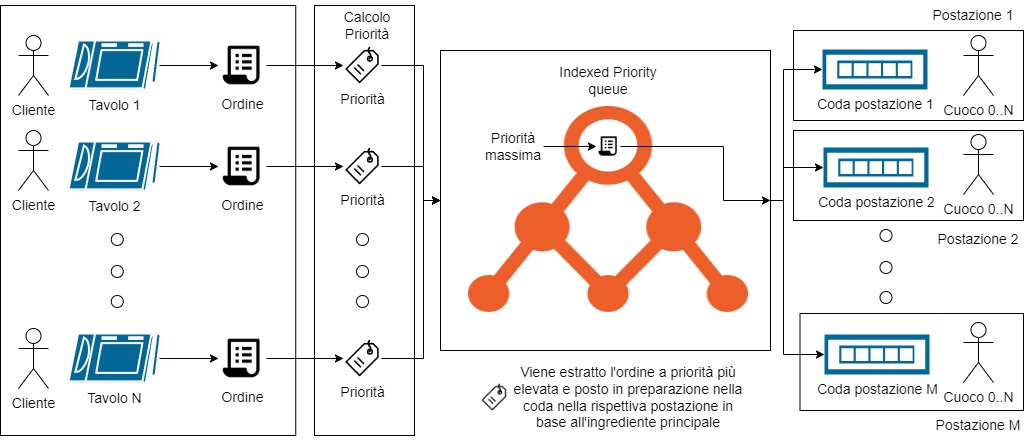
\includegraphics[scale=0.4]{iterazione1/images/Algoritmo_struttura.jpg}
	\caption{Strutture dati dell'algoritmo\label{fig:algoritmo_struttura}}
\end{figure}

Si rendono quindi necessarie due tipi di strutture dati:
\begin{itemize}
	\item Struttura dati principale: Indexed priority queue;
	\item Struttura dati delle postazioni: Coda (queue).
\end{itemize}

\subsection*{Indexed priority queue}
Struttura dati che estende il concetto di coda con priorità aggiungendo la possibilità di accedere in tempo costante agli elementi presenti in coda per compiere operazioni quali la modifica dei parametri, l’aggiornamento della priorità o la rimozione dell’ordine (che altrimenti presenterebbe costo lineare).
Viene implementata per mezzo di una combinazione di una coda con priorità (max heap) e un dizionario (hashtable) che tiene traccia della posizione di ogni elemento all'interno della coda.

\paragraph{Analisi complessità:}
La complessità temporale è correlata a quella di un heap binario, potenziato dall’accesso diretto agli elementi tramite dizionario, di conseguenza:
\begin{itemize}
	\item creazione: O(n);
	\item inserimento e rimozione: O(log n);
	\item modifica priorità: O(log n);
	\item accedere a un elemento: O(1).
\end{itemize}

\paragraph{Requisiti funzionali:}
\begin{itemize}
	\item Gestione degli ordini con priorità: funzionalità chiave della struttura dati, gli ordini ricevono una priorità prima di entrare nella coda a priorità indicizzata;
	\item Fornire l'ordine con priorità più elevata: la struttura dati deve essere in grado di fornire alla cucina l'ordine con la priorità più alta quando richiesto;
	\item Accesso, modifica e rimozione degli ordini: la coda a priorità deve poter fornire la possibilità di implementare la funzionalità che consente ai clienti di accedere, modificare o rimuovere il proprio ordine (nelle prossime iterazioni);
	\item Flessibilità nella modifica delle priorità: la struttura deve garantire una certa flessibilità alla modifica delle priorità degli ordini, poiché le priorità possono cambiare per conto dei clienti, della cucina e a intervalli regolari di tempo.
\end{itemize}

\paragraph{Requisiti non funzionali:}
\begin{itemize}
	\item Tempo di risposta rapido: l’ordine con priorità più elevata deve essere fornito in tempo rapido alla cucina senza ritardi;
	\item Tempo di accesso, modifica e rimozione ragionevole: il cliente deve poter effettuare operazioni senza complicazioni in tempi ragionevoli, mantenendo un’esperienza di utilizzo piacevole;
	\item Scalabilità: La struttura dati deve essere in grado di gestire un grande volume di ordini, adattandosi alle variazioni nella domanda senza compromettere le prestazioni;
	\item Flessibilità alle modifiche: requisito non funzionale relativo alla flessibilità e alla manutenibilità del sistema.
\end{itemize}

\subsection*{Coda (queue)}
Struttura dati lineare che segue il principio "First In, First Out" (FIFO), ossia il principio per il quale il primo elemento che entra nella coda è poi il primo che esce.
\paragraph{Analisi complessità:}
\begin{itemize}
	\item inserimento in coda: O(1);
	\item rimozione della testa: O(1);
	\item verifica stato: O(1) se vuota, O(n) altrimenti.
\end{itemize}

\paragraph{Requisiti funzionali:}
\begin{itemize}
	\item Funzionamento FIFO: La coda deve garantire il corretto funzionamento FIFO (First In, First Out), indipendentemente dalle priorità degli ordini;
	\item Soglia di attivazione: Il sistema deve permettere di configurare una soglia di valore minimo di attivazione per la coda, al di sotto della quale la postazione non viene attivata;
	\item Soglia critica di intasamento: Il sistema deve permettere di configurare una soglia di valore critico, oltre la quale la postazione diventa intasata e richiede operazioni per ridurre il carico.
\end{itemize}

\paragraph{Requisiti non funzionali:}
\begin{itemize}
	\item Lunghezza finita della coda: Il sistema deve gestire una coda con una lunghezza finita, limitata dalla capacità della postazione di lavoro;
	\item Tempo massimo di attesa in coda: Il sistema deve garantire che gli ordini non rimangano in coda di preparazione per troppo tempo prima di essere elaborati;
	\item Attivazione anticipata della postazione: In casi di eccessivo ritardo nella preparazione degli ordini, il sistema può attivare una postazione di lavoro anche se è al di sotto della soglia minima di attivazione.
\end{itemize}

\subsection{Funzione di priorità}
La funzione di priorità è una funzione matematica che assegna un valore numerico decimale di priorità nell’intervallo tra 0 e 1 basandosi sui parametri specifici di ogni ordine.
Il primo passo consiste nel processo di normalizzazione dei parametri, il quale permette di standardizzare i valori in modo che siano compresi tra 0 e 1. in maniera tale da mettere i diversi parametri su una scala comune e uniforme

\subsection*{Parametri}

\paragraph{x1 ingrediente principale:}
Indica il valore di priorità che presenta l'ingrediente predominante dell’ordine, questo valore è influenzato direttamente dallo stato della postazione di lavoro associata in cucina.
\begin{itemize}	
	\item condizione iniziale ogni ingrediente ha valore 0.5
	\item se la cucina è satura ridurre il valore (min 0)
	\item se la cucina è scarica aumentare il valore (max 1)
\end{itemize}

\paragraph{x2 tempo di preparazione:}
Rappresenta la durata stimata necessaria per preparare un determinato ordine.
\begin{itemize}	
	\item normalizzazione: \begin{equation*}
 		\text{tp}_{\text{norm}} = \frac{\text{tp} - \text{tp}_{\text{min}}}{\text{tp}_{\text{max}} - \text{tp}_{\text{min}}}
 	\end{equation*} con tp: tempo di preparazione,\\
 	$\text{tp}_{\text{max}}: \text{tempo di preparazione massimo,}$\\
 	$\text{tp}_{\text{min}}: \text{tempo di preparazione minimo;}$	
	\item $\text{considerare x2 = tp}_{\text{norm}} \text{ per prioritizzare ordini più lunghi,}\\ \text{oppure x2 = 1-tp}_{\text{norm}} \text{ per prioritizzare ordini più brevi.}$
\end{itemize}

\paragraph{x3 urgenza del cliente:}
Consente ai clienti di specificare la tempestività con cui desiderano ricevere il proprio ordine, in particolare i clienti possono chiedere espressamente di avere urgenza, al contrario possono specificare di non avere fretta o non dire nulla e tenere un valore di urgenza di default
\begin{itemize}
	\item 1 se il cliente ha espresso urgenza;
	\item 0 se ha espresso di ritardare o fare con calma;
	\item valore neutro standard 0.5.
\end{itemize}

\paragraph{x4 numero ordine effettuato:}
Specifica il numero dell’ordine del cliente in ordine temporale, in particolare indica la posizione relativa di un ordine all'interno della sequenza di ordini effettuati.
\begin{itemize}
	\item il primo ordine effettuato ha priorità maggiore, mentre i successivi hanno priorità decrescente;
	\item normalizzazione: \begin{equation*}
		\text{x4} = \frac{\text{noe} - 1}{\text{max}_{\text{noe}} - 1}
	\end{equation*} con noe: numero ordini effettuati,\\
	$\text{max}_{\text{noe}} \text{: massimo numero ordini effettuabili;}$
	\item considerare un valore massimo di ordini (es.5 gli ordini dopo il quinto sono comunque consentiti e prenderanno la stessa priorità del 5° ordine).
\end{itemize}

\paragraph{x5 tempo in attesa:}
Rappresenta il periodo di tempo trascorso da quando un ordine è stato effettuato fino al momento in cui viene elaborato.
\begin{itemize}
	\item normalizzazione: \begin{equation*}
		\text{x5} = \frac{\text{tempo in attesa}}{\text{tempo max in attesa}}
	\end{equation*}
	\item considerare un valore massimo di tempo in attesa consentito, in prossimità del quale si ha la priorità più elevata.
\end{itemize}

\subsection*{Pesi}
I pesi sono utilizzati per attribuire un grado di importanza relativo a ciascun parametro all'interno della funzione di priorità. Questi pesi indicano quanto ciascun parametro dovrebbe influenzare il calcolo complessivo della priorità di un determinato elemento.
Si elencano di seguito i pesi per ciascun parametro definito poc’anzi:
\begin{itemize}
	\item p1: peso ingrediente principale;
	\item p2: peso tempo di preparazione;
	\item p3: peso urgenza cliente;
	\item p4: peso numero ordine;
	\item p5: peso tempo in attesa.
\end{itemize}

Viene quindi fatto un ragionamento sull’importanza da attribuire a ogni parametro tramite l’incidenza assegnata al singolo peso. Si dividono quindi i pesi in tre categorie.

\paragraph{Maggiore incidenza} I pesi che devono essere più incidenti sono:
\begin{itemize}
	\item p1 peso ingrediente principale: per evitare di sovraccaricare una postazione rispetto alle altre o per non avere postazioni vuote;
	\item p5 peso tempo in attesa: un ordine non può restare in attesa troppo a lungo.
\end{itemize}

\paragraph{Incidenza media} Il peso con incidenza media è:
\begin{itemize}
	\item p3 peso urgenza del cliente: è meno importante dei vincoli di sovraccarico e attesa, ma deve essere comunque una scelta significativa.
\end{itemize}

\paragraph{Bassa incidenza} I pesi con bassa incidenza sulla priorità sono:
\begin{itemize}
	\item p2 peso tempo di preparazione: in confronto ad altri parametri con pesi più elevati, questo è considerato meno critico;
	\item p4 peso numero ordine effettuato: ha un impatto di poco conto sulla priorità dell’ordine.
\end{itemize}

\subsubsection*{Valore dei pesi}
I valori dei pesi vengono quindi definiti inizialmente:
\begin{itemize}
	\item p1 = 0.25;
	\item p2 = 0.15;
	\item p3 = 0.20;
	\item p4 = 0.15;
	\item p5 = 0.25.
\end{itemize}
Questi valori possono essere regolati col tempo per aumentare l’efficienza dell’algoritmo, diventa così importante raccogliere dati storici per poterli analizzare e comprendere come i vari parametri influenzano le prestazioni del sistema, oltre a raccogliere feedback dei clienti, sulla base di ciò sarà richiesto un tuning dei pesi più accurato. Per questo motivo è richiesta una certa flessibilità in modo da consentire l'aggiornamento dei pesi dei parametri in modo dinamico.

\subsection*{Funzione matematica}
L'equazione proposta rappresenta una somma pesata dei parametri, dove ciascun parametro (x1, x2, x3, x4, x5) viene moltiplicato per il suo relativo peso (p1, p2, p3, p4, p5). I pesi indicano l'importanza relativa dei parametri nel determinare la priorità complessiva di un elemento. La somma pesata dei parametri produce un valore (y) compreso tra 0 e 1, dove 0 indica un valore meno urgente e 1 indica un valore più urgente.
\begin{equation*}
	\text{y} = \text{p1}*{\text{x1}} + \text{p2}*{\text{x2}}  + \text{p3}*{\text{x3}}  + \text{p4}*{\text{x4}}  + \text{p5}*{\text{x5}} 
\end{equation*}

\subsection{Diagramma di flusso}
Per comprendere meglio il processo dell’algoritmo viene mostrato il diagramma di flusso in \figurename~\ref{fig:flowchart}, nel quale viene mostrato il flusso di un ordine dal momento in cui viene effettuato dal cliente a quando viene assegnato alla postazione di lavoro in cucina.
\begin{figure}[htbp]
	\centering
	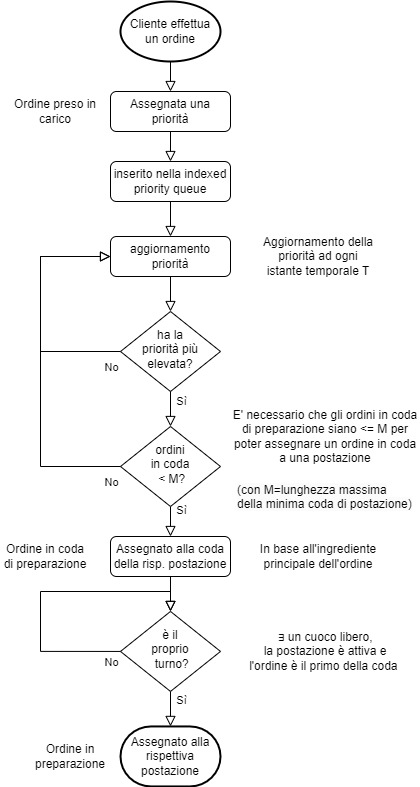
\includegraphics[scale=0.7]{iterazione1/images/flowchart.jpg}
	\caption{Diagramma di flusso\label{fig:flowchart}}
\end{figure}
	\backmatter	
	
\end{document}